%!TEX root = ../report.tex

\chapter{Experiments}

\picHereWidth{experimental_setup}{Experiment setup: the robot assumes the same pose before each grasp.}
             {fig:experiment_setup}{0.7\textwidth}

\begin{figure}[htb]
    \centering
    \small
    \begin{subfigure}[b]{0.45\textwidth}
        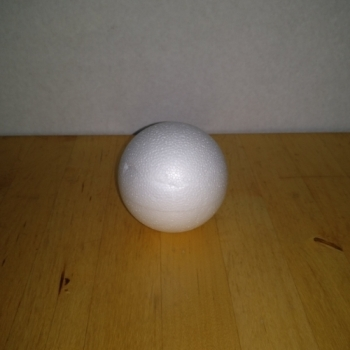
\includegraphics[width=\textwidth]{object_ball}
        \caption{A white styrofoam ball}
        \label{fig:object_ball}
    \end{subfigure}
    \hfill
    \begin{subfigure}[b]{0.45\textwidth}
        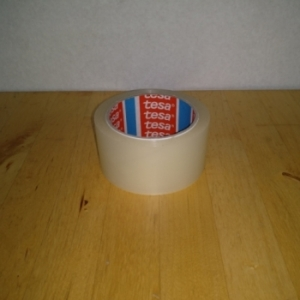
\includegraphics[width=\textwidth]{object_duct_tape}
        \caption{A roll of duct tape}
        \label{fig:object_duct_tape}
    \end{subfigure}
    
    \begin{subfigure}[b]{0.45\textwidth}
        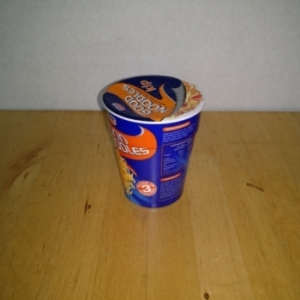
\includegraphics[width=\textwidth]{object_noodle_box}
        \caption{A cup noodles box}
        \label{fig:object_noodle_box}
    \end{subfigure}
    \hfill
    \begin{subfigure}[b]{0.45\textwidth}
        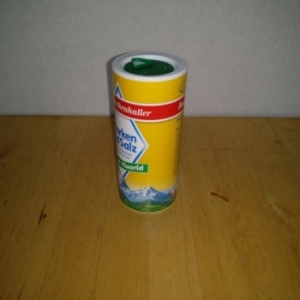
\includegraphics[width=\textwidth]{object_salt}
        \caption{A salt container}
        \label{fig:object_salt}
    \end{subfigure}
    \caption{Objects selected for the experiments.}\label{fig:objects}
\end{figure}

\section{Setup}

\section{Experimental Design}
